\section{Nearest Neighbor Analysis}
\begin{frame}
\frametitle{Nearest Neighbor Analysis}
\tikzproblem{Given the ET value of $k$ nearest stations of a place, can we estimate ET?}
\onslide<2>{
\begin{itemize}
\setlength\itemsep{1em}
\item Arithmetic mean of $k$ values
\item Inverse Distance Weighted (IDW) average of $k$ values
\end{itemize}
}
\end{frame}

\begin{frame}
\begin{figure}
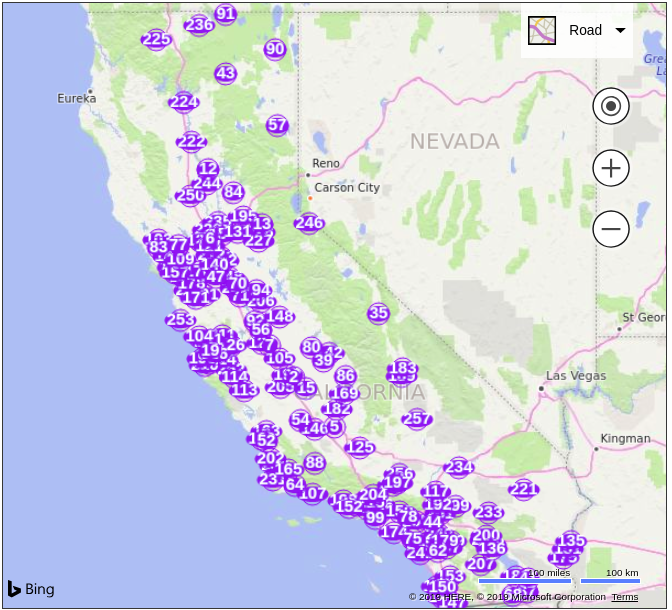
\includegraphics[width=0.8\textwidth]{images/cimis-station-location}
\end{figure}
\end{frame}

\begin{frame}
\frametitle{Stations of Interest}
\begin{itemize}
	\setlength\itemsep{1em}
	\item Station with lowest distance $D_{MIN}$ to nearest neighbor
	\item Station with highest distance $D_{MAX}$ to nearest neighbor
	\item Station with nearest neighbor at a distance closest to $\frac{D_{MIN}+D_{MAX}}{2}$
\end{itemize}
\end{frame}

\begin{frame}
\frametitle{Nearest Neighbor Results}
\centering
\footnotesize
\begin{tabular}{|l|l|l|l|}
\hline
\textbf{Station Number} & \textbf{Num of Neighbors} & \textbf{MSE for Average} &\textbf{MSE for IDW}\\
\hline
129 & 1 & 0.000832971114168 & 0.000832971114168\\
\hline
234 & 1 & 0.00437018526497 & 0.00437018526497\\
\hline
57 & 1 & 0.00451400872516 & 0.00451400872516\\
\hline
129 & 2 & 0.00116361600992 & 0.000620877927137\\
\hline
234 & 2 & 0.00761026004119 & 0.00730456269316\\
\hline
57 & 2 & 0.00371994564336 & 0.0037154634375\\
\hline
129 & 3 & 0.000890784115612 & 0.000596760525931\\
\hline
234 & 3 & 0.00908058999082 & 0.00863260116925\\
\hline
57 & 3 & 0.00335367604618 & 0.00334925237208\\
\hline
129 & 4 & 0.00116647617403 & 0.00063999172153\\
\hline
234 & 4 & 0.00919325287807 & 0.00878339044833\\
\hline
57 & 4 & 0.00361403432169 & 0.00357201358681\\
\hline
\end{tabular}
\end{frame}

\begin{frame}
\begin{figure}
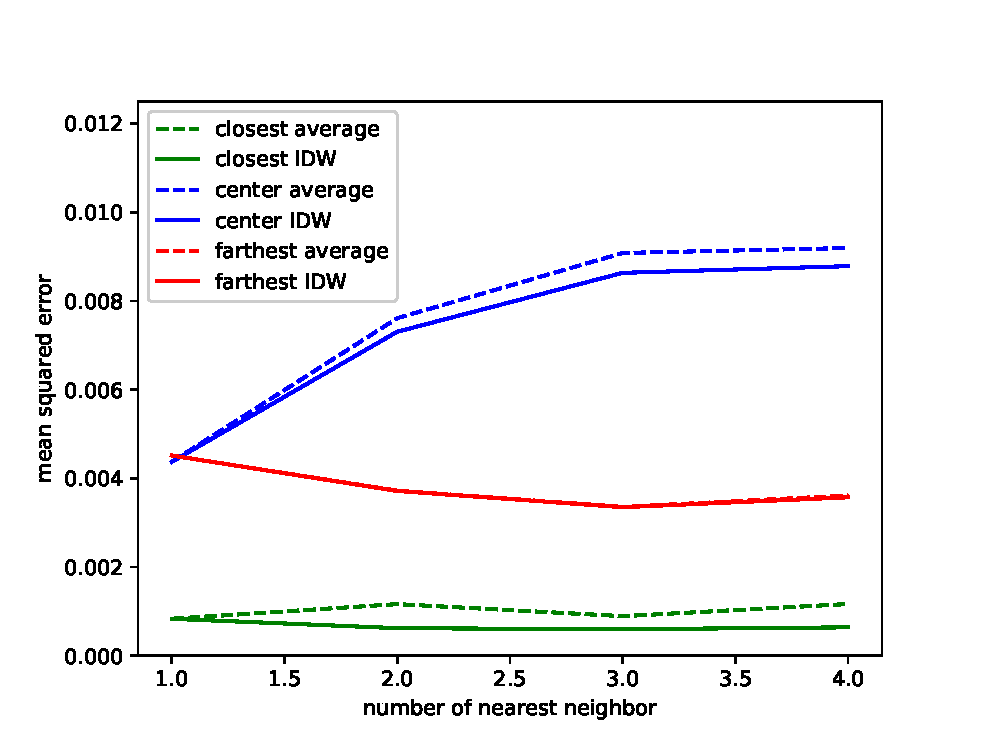
\includegraphics[width=1.0\textwidth]{images/soi-nearest-distance}
\end{figure}
\end{frame}

\begin{frame}
\frametitle{Nearest Neighbor with Sensor Values}
\onslide<1->{\tikzproblem{What if we have sensor values from nearby stations instead of only ET values?}}
\onslide<2->{\tikzsolution{MSE decreases according to CIMIS Penman Equation}}
~\\
\onslide<3->{\tikzproblem{What if we have sensor values from nearby stations \textbf{along with local air temperature?}}}
\onslide<4>{\tikzsolution{MSE decreases even further}}
\end{frame}

\begin{frame}
\frametitle{Nearest Neighbor with Sensor Values \continued}
\centering
\begin{tabular}{|l|l|l|l|l|}
\hline
	\textbf{Stn No} & \textbf{Num of Nbrs} & \textbf{MSE IDW} & \textbf{MSE} &\textbf{MSE Local}\\
\hline
234 & 1 & 0.00437018 & 0.00085818 & 0.00001899\\
\hline
234 & 2 & 0.00730456 & 0.00401320 & 0.00002029\\
\hline
234 & 3 & 0.00863260 & 0.00480052 & 0.00002029\\
\hline
234 & 4 & 0.00878339 & 0.00284048 & 0.00002034\\
\hline
129 & 1 & 0.00083297 & 0.00023209 & 0.00000650\\
\hline
129 & 2 & 0.00062087 & 0.00037144 & 0.00000649\\
\hline
129 & 3 & 0.00059676 & 0.00028950 & 0.00000649\\
\hline
129 & 4 & 0.00063999 & 0.00042391 & 0.00000650\\
\hline
57 & 1 & 0.00451400 & 0.00044228 & 0.00000982\\
\hline
57 & 2 & 0.00371546 & 0.00051686 & 0.00000982\\
\hline
57 & 3 & 0.00334925 & 0.00031521 & 0.00000982\\
\hline
57 & 4 & 0.00357201 & 0.00042077 & 0.00000983\\
\hline
\end{tabular}
\end{frame}

\begin{frame}
\frametitle{Nearest Neighbor with Sensor Values \continued}
\centering
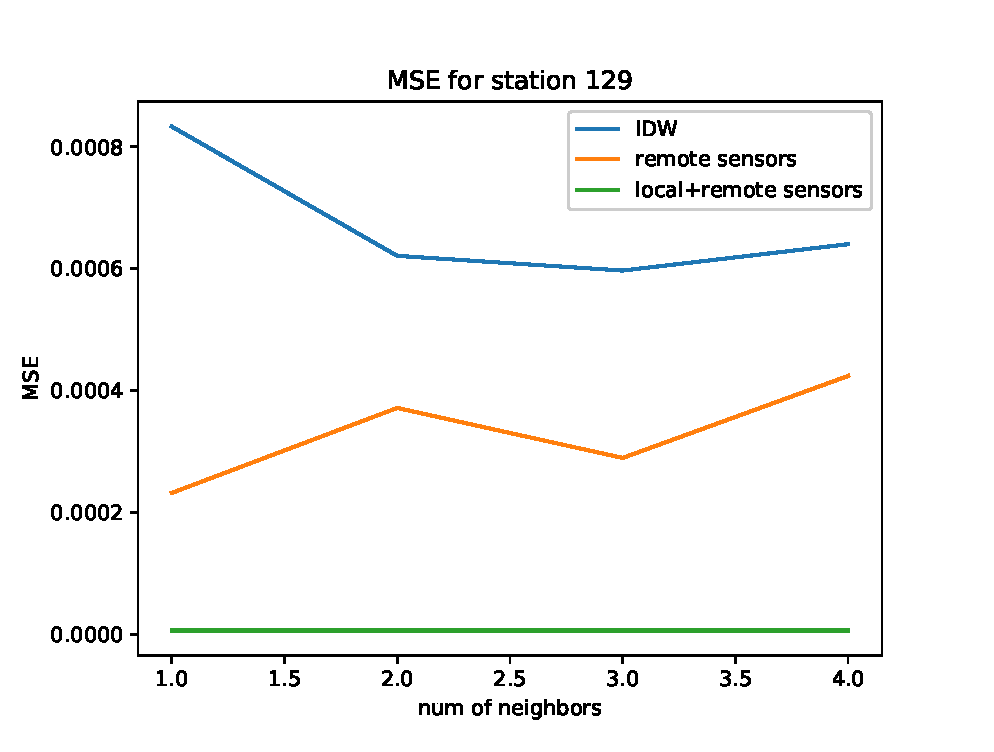
\includegraphics[width=0.9\textwidth]{images/129-idw-local-remote}
\end{frame}

\begin{frame}
\frametitle{Nearest Neighbor with Sensor Values \continued}
\centering
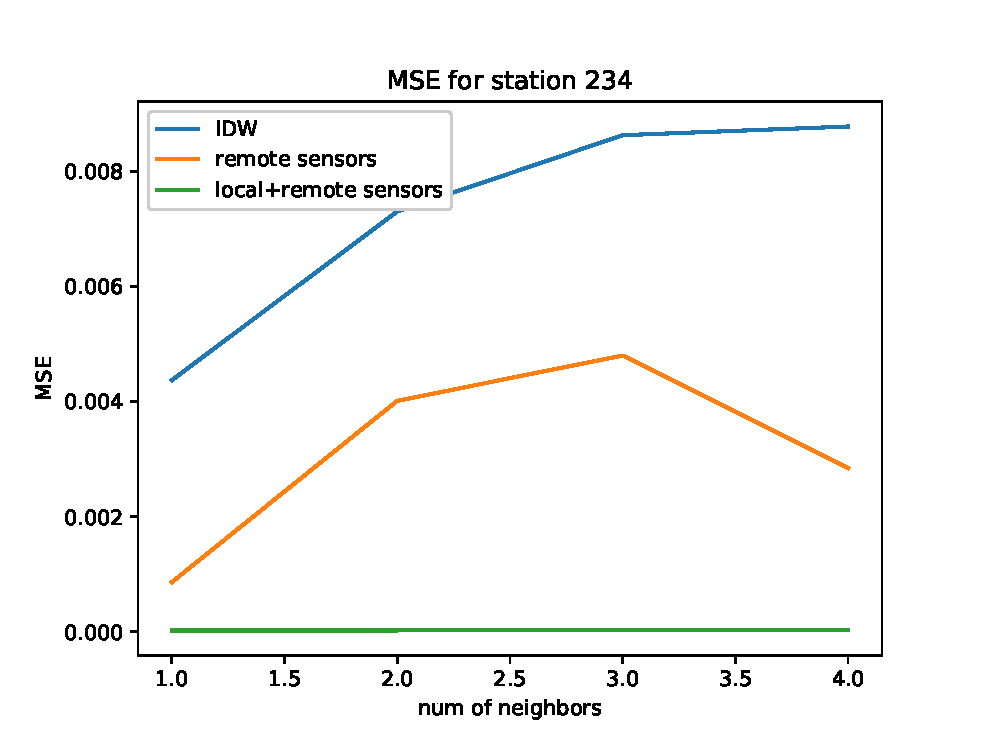
\includegraphics[width=0.9\textwidth]{images/234-idw-local-remote}
\end{frame}

\begin{frame}
\frametitle{Nearest Neighbor with Sensor Values \continued}
\centering
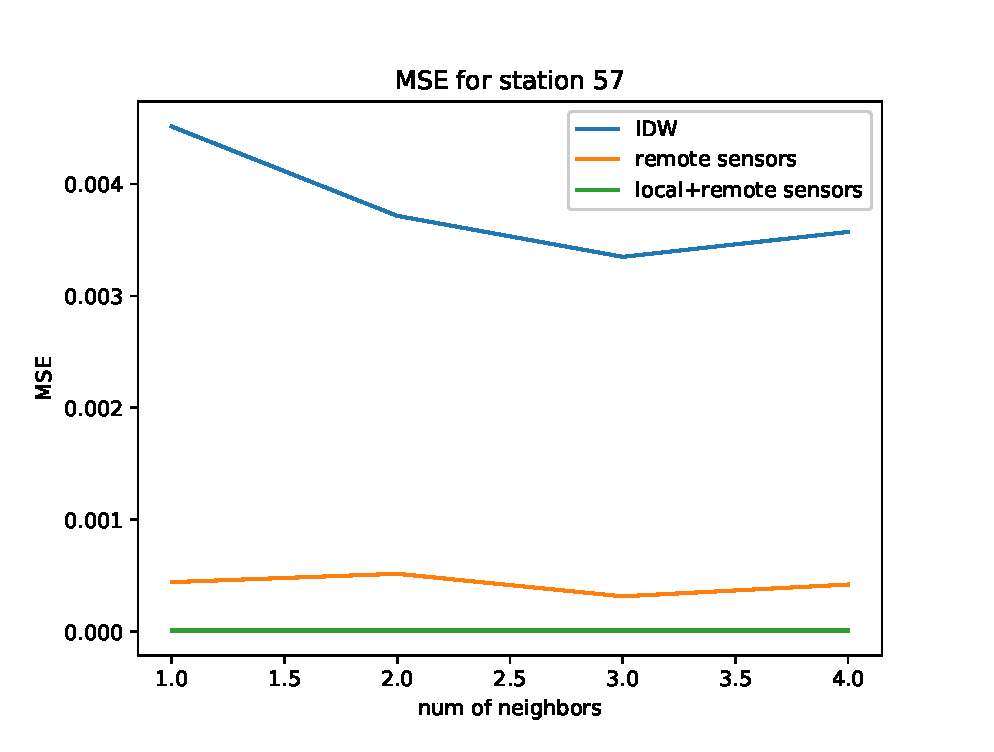
\includegraphics[width=0.9\textwidth]{images/57-idw-local-remote}
\end{frame}

%\begin{frame}
%\frametitle{A Different Approach to Nearest Neighbor}
%\begin{itemize}
%\setlength\itemsep{1em}
%\item Some stations are sparsely located, some are densely located
%\item Distance to $n$th nearest station for different stations might vary widely
%\end{itemize}
%\onslide<2>{
%\tikzproblem{What is an optimal value of radius $R$ such that $k\prime$ stations\\ within that radius gives best overall estimates?}
%\tikzsolution{Future Work$\ldots$}
%}
%\end{frame}
